% Options for packages loaded elsewhere
\PassOptionsToPackage{unicode}{hyperref}
\PassOptionsToPackage{hyphens}{url}
%
\documentclass[
  12 pt,
  a4paper,
]{article}
\usepackage{amsmath,amssymb}
\usepackage{setspace}
\usepackage{iftex}
\ifPDFTeX
  \usepackage[T1]{fontenc}
  \usepackage[utf8]{inputenc}
  \usepackage{textcomp} % provide euro and other symbols
\else % if luatex or xetex
  \usepackage{unicode-math} % this also loads fontspec
  \defaultfontfeatures{Scale=MatchLowercase}
  \defaultfontfeatures[\rmfamily]{Ligatures=TeX,Scale=1}
\fi
\usepackage{lmodern}
\ifPDFTeX\else
  % xetex/luatex font selection
  \setmainfont[]{Times New Roman}
\fi
% Use upquote if available, for straight quotes in verbatim environments
\IfFileExists{upquote.sty}{\usepackage{upquote}}{}
\IfFileExists{microtype.sty}{% use microtype if available
  \usepackage[]{microtype}
  \UseMicrotypeSet[protrusion]{basicmath} % disable protrusion for tt fonts
}{}
\makeatletter
\@ifundefined{KOMAClassName}{% if non-KOMA class
  \IfFileExists{parskip.sty}{%
    \usepackage{parskip}
  }{% else
    \setlength{\parindent}{0pt}
    \setlength{\parskip}{6pt plus 2pt minus 1pt}}
}{% if KOMA class
  \KOMAoptions{parskip=half}}
\makeatother
\usepackage{xcolor}
\usepackage[margin=1in]{geometry}
\usepackage{color}
\usepackage{fancyvrb}
\newcommand{\VerbBar}{|}
\newcommand{\VERB}{\Verb[commandchars=\\\{\}]}
\DefineVerbatimEnvironment{Highlighting}{Verbatim}{commandchars=\\\{\}}
% Add ',fontsize=\small' for more characters per line
\usepackage{framed}
\definecolor{shadecolor}{RGB}{248,248,248}
\newenvironment{Shaded}{\begin{snugshade}}{\end{snugshade}}
\newcommand{\AlertTok}[1]{\textcolor[rgb]{0.94,0.16,0.16}{#1}}
\newcommand{\AnnotationTok}[1]{\textcolor[rgb]{0.56,0.35,0.01}{\textbf{\textit{#1}}}}
\newcommand{\AttributeTok}[1]{\textcolor[rgb]{0.13,0.29,0.53}{#1}}
\newcommand{\BaseNTok}[1]{\textcolor[rgb]{0.00,0.00,0.81}{#1}}
\newcommand{\BuiltInTok}[1]{#1}
\newcommand{\CharTok}[1]{\textcolor[rgb]{0.31,0.60,0.02}{#1}}
\newcommand{\CommentTok}[1]{\textcolor[rgb]{0.56,0.35,0.01}{\textit{#1}}}
\newcommand{\CommentVarTok}[1]{\textcolor[rgb]{0.56,0.35,0.01}{\textbf{\textit{#1}}}}
\newcommand{\ConstantTok}[1]{\textcolor[rgb]{0.56,0.35,0.01}{#1}}
\newcommand{\ControlFlowTok}[1]{\textcolor[rgb]{0.13,0.29,0.53}{\textbf{#1}}}
\newcommand{\DataTypeTok}[1]{\textcolor[rgb]{0.13,0.29,0.53}{#1}}
\newcommand{\DecValTok}[1]{\textcolor[rgb]{0.00,0.00,0.81}{#1}}
\newcommand{\DocumentationTok}[1]{\textcolor[rgb]{0.56,0.35,0.01}{\textbf{\textit{#1}}}}
\newcommand{\ErrorTok}[1]{\textcolor[rgb]{0.64,0.00,0.00}{\textbf{#1}}}
\newcommand{\ExtensionTok}[1]{#1}
\newcommand{\FloatTok}[1]{\textcolor[rgb]{0.00,0.00,0.81}{#1}}
\newcommand{\FunctionTok}[1]{\textcolor[rgb]{0.13,0.29,0.53}{\textbf{#1}}}
\newcommand{\ImportTok}[1]{#1}
\newcommand{\InformationTok}[1]{\textcolor[rgb]{0.56,0.35,0.01}{\textbf{\textit{#1}}}}
\newcommand{\KeywordTok}[1]{\textcolor[rgb]{0.13,0.29,0.53}{\textbf{#1}}}
\newcommand{\NormalTok}[1]{#1}
\newcommand{\OperatorTok}[1]{\textcolor[rgb]{0.81,0.36,0.00}{\textbf{#1}}}
\newcommand{\OtherTok}[1]{\textcolor[rgb]{0.56,0.35,0.01}{#1}}
\newcommand{\PreprocessorTok}[1]{\textcolor[rgb]{0.56,0.35,0.01}{\textit{#1}}}
\newcommand{\RegionMarkerTok}[1]{#1}
\newcommand{\SpecialCharTok}[1]{\textcolor[rgb]{0.81,0.36,0.00}{\textbf{#1}}}
\newcommand{\SpecialStringTok}[1]{\textcolor[rgb]{0.31,0.60,0.02}{#1}}
\newcommand{\StringTok}[1]{\textcolor[rgb]{0.31,0.60,0.02}{#1}}
\newcommand{\VariableTok}[1]{\textcolor[rgb]{0.00,0.00,0.00}{#1}}
\newcommand{\VerbatimStringTok}[1]{\textcolor[rgb]{0.31,0.60,0.02}{#1}}
\newcommand{\WarningTok}[1]{\textcolor[rgb]{0.56,0.35,0.01}{\textbf{\textit{#1}}}}
\usepackage{longtable,booktabs,array}
\usepackage{calc} % for calculating minipage widths
% Correct order of tables after \paragraph or \subparagraph
\usepackage{etoolbox}
\makeatletter
\patchcmd\longtable{\par}{\if@noskipsec\mbox{}\fi\par}{}{}
\makeatother
% Allow footnotes in longtable head/foot
\IfFileExists{footnotehyper.sty}{\usepackage{footnotehyper}}{\usepackage{footnote}}
\makesavenoteenv{longtable}
\usepackage{graphicx}
\makeatletter
\def\maxwidth{\ifdim\Gin@nat@width>\linewidth\linewidth\else\Gin@nat@width\fi}
\def\maxheight{\ifdim\Gin@nat@height>\textheight\textheight\else\Gin@nat@height\fi}
\makeatother
% Scale images if necessary, so that they will not overflow the page
% margins by default, and it is still possible to overwrite the defaults
% using explicit options in \includegraphics[width, height, ...]{}
\setkeys{Gin}{width=\maxwidth,height=\maxheight,keepaspectratio}
% Set default figure placement to htbp
\makeatletter
\def\fps@figure{htbp}
\makeatother
\setlength{\emergencystretch}{3em} % prevent overfull lines
\providecommand{\tightlist}{%
  \setlength{\itemsep}{0pt}\setlength{\parskip}{0pt}}
\setcounter{secnumdepth}{-\maxdimen} % remove section numbering
\ifLuaTeX
\usepackage[bidi=basic]{babel}
\else
\usepackage[bidi=default]{babel}
\fi
\babelprovide[main,import]{spanish}
\ifPDFTeX
\else
\babelfont{rm}[]{Times New Roman}
\fi
% get rid of language-specific shorthands (see #6817):
\let\LanguageShortHands\languageshorthands
\def\languageshorthands#1{}
\ifLuaTeX
  \usepackage{selnolig}  % disable illegal ligatures
\fi
\usepackage{bookmark}
\IfFileExists{xurl.sty}{\usepackage{xurl}}{} % add URL line breaks if available
\urlstyle{same}
\hypersetup{
  pdflang={es-ES},
  hidelinks,
  pdfcreator={LaTeX via pandoc}}

\title{U7-ADMINISTRACIÓ DE SISTEMA OPERATIUS}
\usepackage{etoolbox}
\makeatletter
\providecommand{\subtitle}[1]{% add subtitle to \maketitle
  \apptocmd{\@title}{\par {\large #1 \par}}{}{}
}
\makeatother
\subtitle{~Comprovar sha256sum}
\author{}
\date{\vspace{-2.5em}}

\begin{document}
\maketitle

\setstretch{1.5}
\section{1 CODI HASH}\label{codi-hash}

Un codi hash és un valor únic generat a partir de dades mitjançant un
algorisme matemàtic. Serveix per identificar i verificar informació
sense revelar-ne el contingut.

\subsection{1.1 Característiques:}\label{caracteruxedstiques}

\begin{itemize}
\item
  De mida fixa (ex: 256 bits per SHA-256).
\item
  Un petit canvi a les dades genera un hash completament diferent.
\item
  No es pot revertir (no es pot obtenir l'original des del hash).
\end{itemize}

\subsection{1.2 Usos:}\label{usos}

\begin{itemize}
\item
  \textbf{Verificació de fitxers (integritat)}
\item
  Emmagatzematge segur de contrasenyes.
\item
  Signatures digitals i seguretat informàtica.
\end{itemize}

\subsubsection{Exemples de diferents
algorismes:}\label{exemples-de-diferents-algorismes}

En negreta resalte el que anem a usar.

\begin{longtable}[]{@{}
  >{\raggedright\arraybackslash}p{(\columnwidth - 6\tabcolsep) * \real{0.2264}}
  >{\raggedright\arraybackslash}p{(\columnwidth - 6\tabcolsep) * \real{0.3208}}
  >{\raggedright\arraybackslash}p{(\columnwidth - 6\tabcolsep) * \real{0.2075}}
  >{\raggedright\arraybackslash}p{(\columnwidth - 6\tabcolsep) * \real{0.2453}}@{}}
\toprule\noalign{}
\begin{minipage}[b]{\linewidth}\raggedright
Algorisme
\end{minipage} & \begin{minipage}[b]{\linewidth}\raggedright
Longitud del hash
\end{minipage} & \begin{minipage}[b]{\linewidth}\raggedright
Seguretat
\end{minipage} & \begin{minipage}[b]{\linewidth}\raggedright
Ús principal
\end{minipage} \\
\midrule\noalign{}
\endhead
\bottomrule\noalign{}
\endlastfoot
MD5 & 128 bits (32 caràcters) & Feble (col·lisions) & Comprovació de
fitxers (no segur per criptografia) \\
SHA-1 & 160 bits (40 caràcters) & Feble (col·lisions trobades) &
Signatures digitals antigues \\
\textbf{SHA-256} & 256 bits (64 caràcters) & Alta & Certificats
digitals, blockchain, \textbf{integritat de dades} \\
SHA-512 & 512 bits (128 caràcters) & Molt alta & Seguretat avançada \\
BLAKE2 & 256-512 bits & Més ràpid que SHA-256 & Criptografia moderna \\
Argon2 & Variable & Molt segura & Emmagatzematge de contrasenyes \\
bcrypt & 192 bits & Resistència a atacs de força bruta & Protecció de
contrasenyes \\
\end{longtable}

\section{\texorpdfstring{2.- SHA256 en LINUX:
\emph{sha256sum}}{2.- SHA256 en LINUX: sha256sum}}\label{sha256-en-linux-sha256sum}

\begin{itemize}
\tightlist
\item
  Llegeix les dades d'un fitxer o entrada.
\item
  Processa les dades mitjançant l'algorisme SHA-256.
\item
  Retorna una cadena hexadecimal de 64 caràcters que representa el hash.
\end{itemize}

Exemple:

\begin{Shaded}
\begin{Highlighting}[]
\FunctionTok{sha256sum}\NormalTok{ exemple.txt}
\ExtensionTok{5e884898da28047151d0e56f8dc6292773603d0d6aabbdd89c6b247dd60a8a6e}\NormalTok{  exemple.txt}
\end{Highlighting}
\end{Shaded}

\subsection{2.1 Verificació de una ISO}\label{verificaciuxf3-de-una-iso}

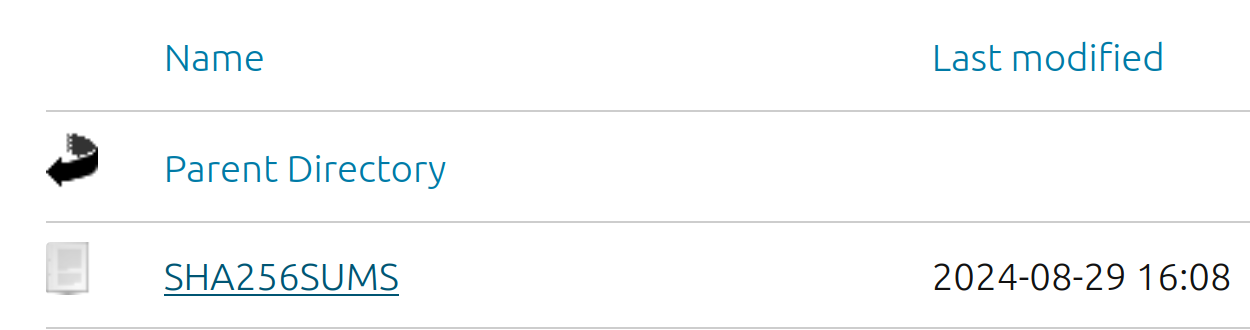
\includegraphics{png/sha256-1.png}

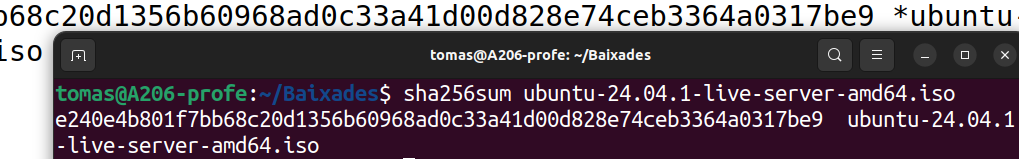
\includegraphics{png/sha256-2.png}

\section{3. SHA256 en WINDOWS}\label{sha256-en-windows}

\subsection{3.1 Informació}\label{informaciuxf3}

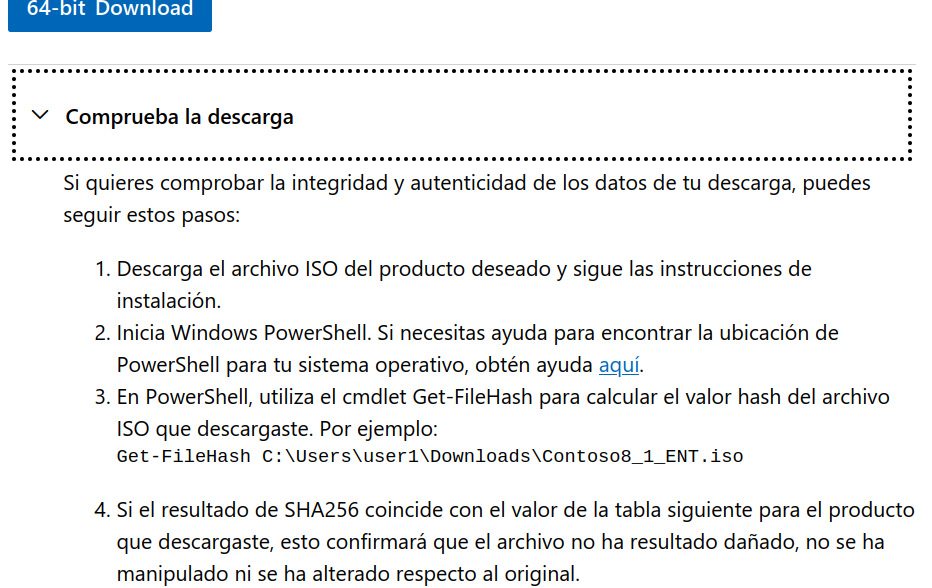
\includegraphics{png/sha256Windows-1.png}

\subsection{3.2 Get-FileHash}\label{get-filehash}

\begin{Shaded}
\begin{Highlighting}[]
\NormalTok{Get{-}FileHash }\OperatorTok{{-}}\NormalTok{Path }\StringTok{"C:\textbackslash{}Windows.iso"} \OperatorTok{{-}}\NormalTok{Algorithm SHA256}
\end{Highlighting}
\end{Shaded}

Ens donarà, per exemple:

\begin{verbatim}
Algorithm       Hash                                                                   Path
---------       ----                                                                   ----
SHA256         0D48C6F236CA9F966ECCD84D9BE01B038516567AABF1C46DCBEE785556B19813       C:\Ruta\Windows.iso
\end{verbatim}

En Windows tenim un codi Hash (sha256) distint per cada idioma:

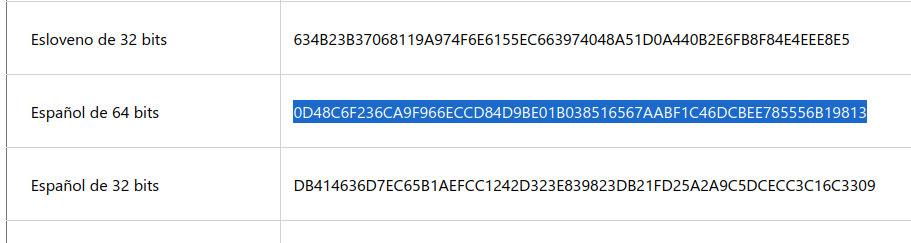
\includegraphics{png/sha256Windows-3.png}

Comprovem que els codis coincideixen.

\section{4 ALTRES USOS}\label{altres-usos}

Encara que el cas de les ISO de Sistemes Operatius serà l'ús més
habitual en quant a la verificació de la \textbf{integritat d'un fitxer}
pode donar altres usos.

Exemple: Ens demanen que compartim en un portal web un fitxer gran que
altri podrà descarregar mitjaçant https o ftp. Podem generar el codi
\emph{sha256} i compartir-lo per a que, després de la descàrrega es
puguen comprovar si ha anat bé.

\begin{Shaded}
\begin{Highlighting}[]
\ExtensionTok{tomas@portatil:\textasciitilde{}$}\NormalTok{ sha256sum smartgit{-}linux{-}23\_1\_2.tar.gz}\OperatorTok{\textgreater{}\textgreater{}}\NormalTok{sha256sum.txt}
\ExtensionTok{tomas@portatil:\textasciitilde{}$}\NormalTok{ ls }\AttributeTok{{-}l}\NormalTok{ sha256sum.txt}
\ExtensionTok{{-}rw{-}rw{-}r{-}{-}}\NormalTok{ 1 tomas tomas 95 de gen.  29 12:01 sha256sum.txt}
\end{Highlighting}
\end{Shaded}

És indistint que usem Linux (sha256sum) que usem cmdLets (Get-FileHash).
La funció \emph{sha256} és la mateixa.

\end{document}
